\newpage

\chapter{Desarrollo software }
\chaptermark{desarrollo}
\label{chap:desarrollo-software}


\section{Metodología de desarrollo}

Este proyecto ha sido elaborado empleando una metodología de desarrollo basada en el modelo de desarrollo incremental para la parte software referente a todos los subsistemas web y una metodología de 
desarrollo en cascada para el desarrollo de la parte software referente al robot de pruebas.\\

El modelo de desarrollo incremental proporciona una serie de características que lo hacen idóneo para este proyecto. Dicho modelo se basa en la filosofía de construir 
e ir incrementando las funcionalidades del sistema mediante el desarrollo de los diferentes módulos. Esto permite ir aumentando gradualmente las capacidades del software. \\

Dicha metodología de desarrollo resulta especialmente útil en las siguientes situaciones:\\

\begin{itemize}
 \item Facilita el desarrollo permitiendo a cada miembro del equipo desarrollar un módulo particular. En el caso del presente proyecto me ha permitido desarrollar un módulo tras otro de una manera secuencial.
 \item Es similar al ciclo de vida en cascada aplicándose un ciclo en cada nueva funcionalidad del programa.
 \item A final de cada ciclo se entrega el software al cliente. En el caso que compete a este proyecto se mantenía una reunión con el director del proyecto para su aprobación.
\end{itemize}

Centrándonos nuevamente en el desarrollo del proyecto, los motivos que llevaron a cabo la elección de un modelo de desarrollo incremental viene dada por la necesidad de simplificar e ir
desarrollando de una forma gradual y modularizada debido a la extensión del proyecto. Más si cabe que el equipo de desarrollo solo consta de una persona.\\

Por otro lado, para el desarrollo del vehículo de pruebas y por su simplicidad, se ha optado por un desarrollo en cascada. El modelo de desarrollo en cascada resulta adecuado en situaciones
en las que:\\

\begin{itemize}
 \item Se dispone de unos requisitos claros y precisos.
 \item El sistema a desarrollar es de pequeña envergadura.
 \item Las tecnologías utilizadas son conocidas por los desarrolladores.
\end{itemize}

Siendo precisamente éstas las características del proyecto del vehículo a desarrollar puesto que se trata de un desarrollo de pequeño tamaño y las herramientas empleadas ya me resultaban conocidas
tras la realización de otros trabajos previos.\\

Por tanto el proyecto queda distribuido en los siguientes subsistemas:\\

\begin{figure}[H]
  \begin{center}
    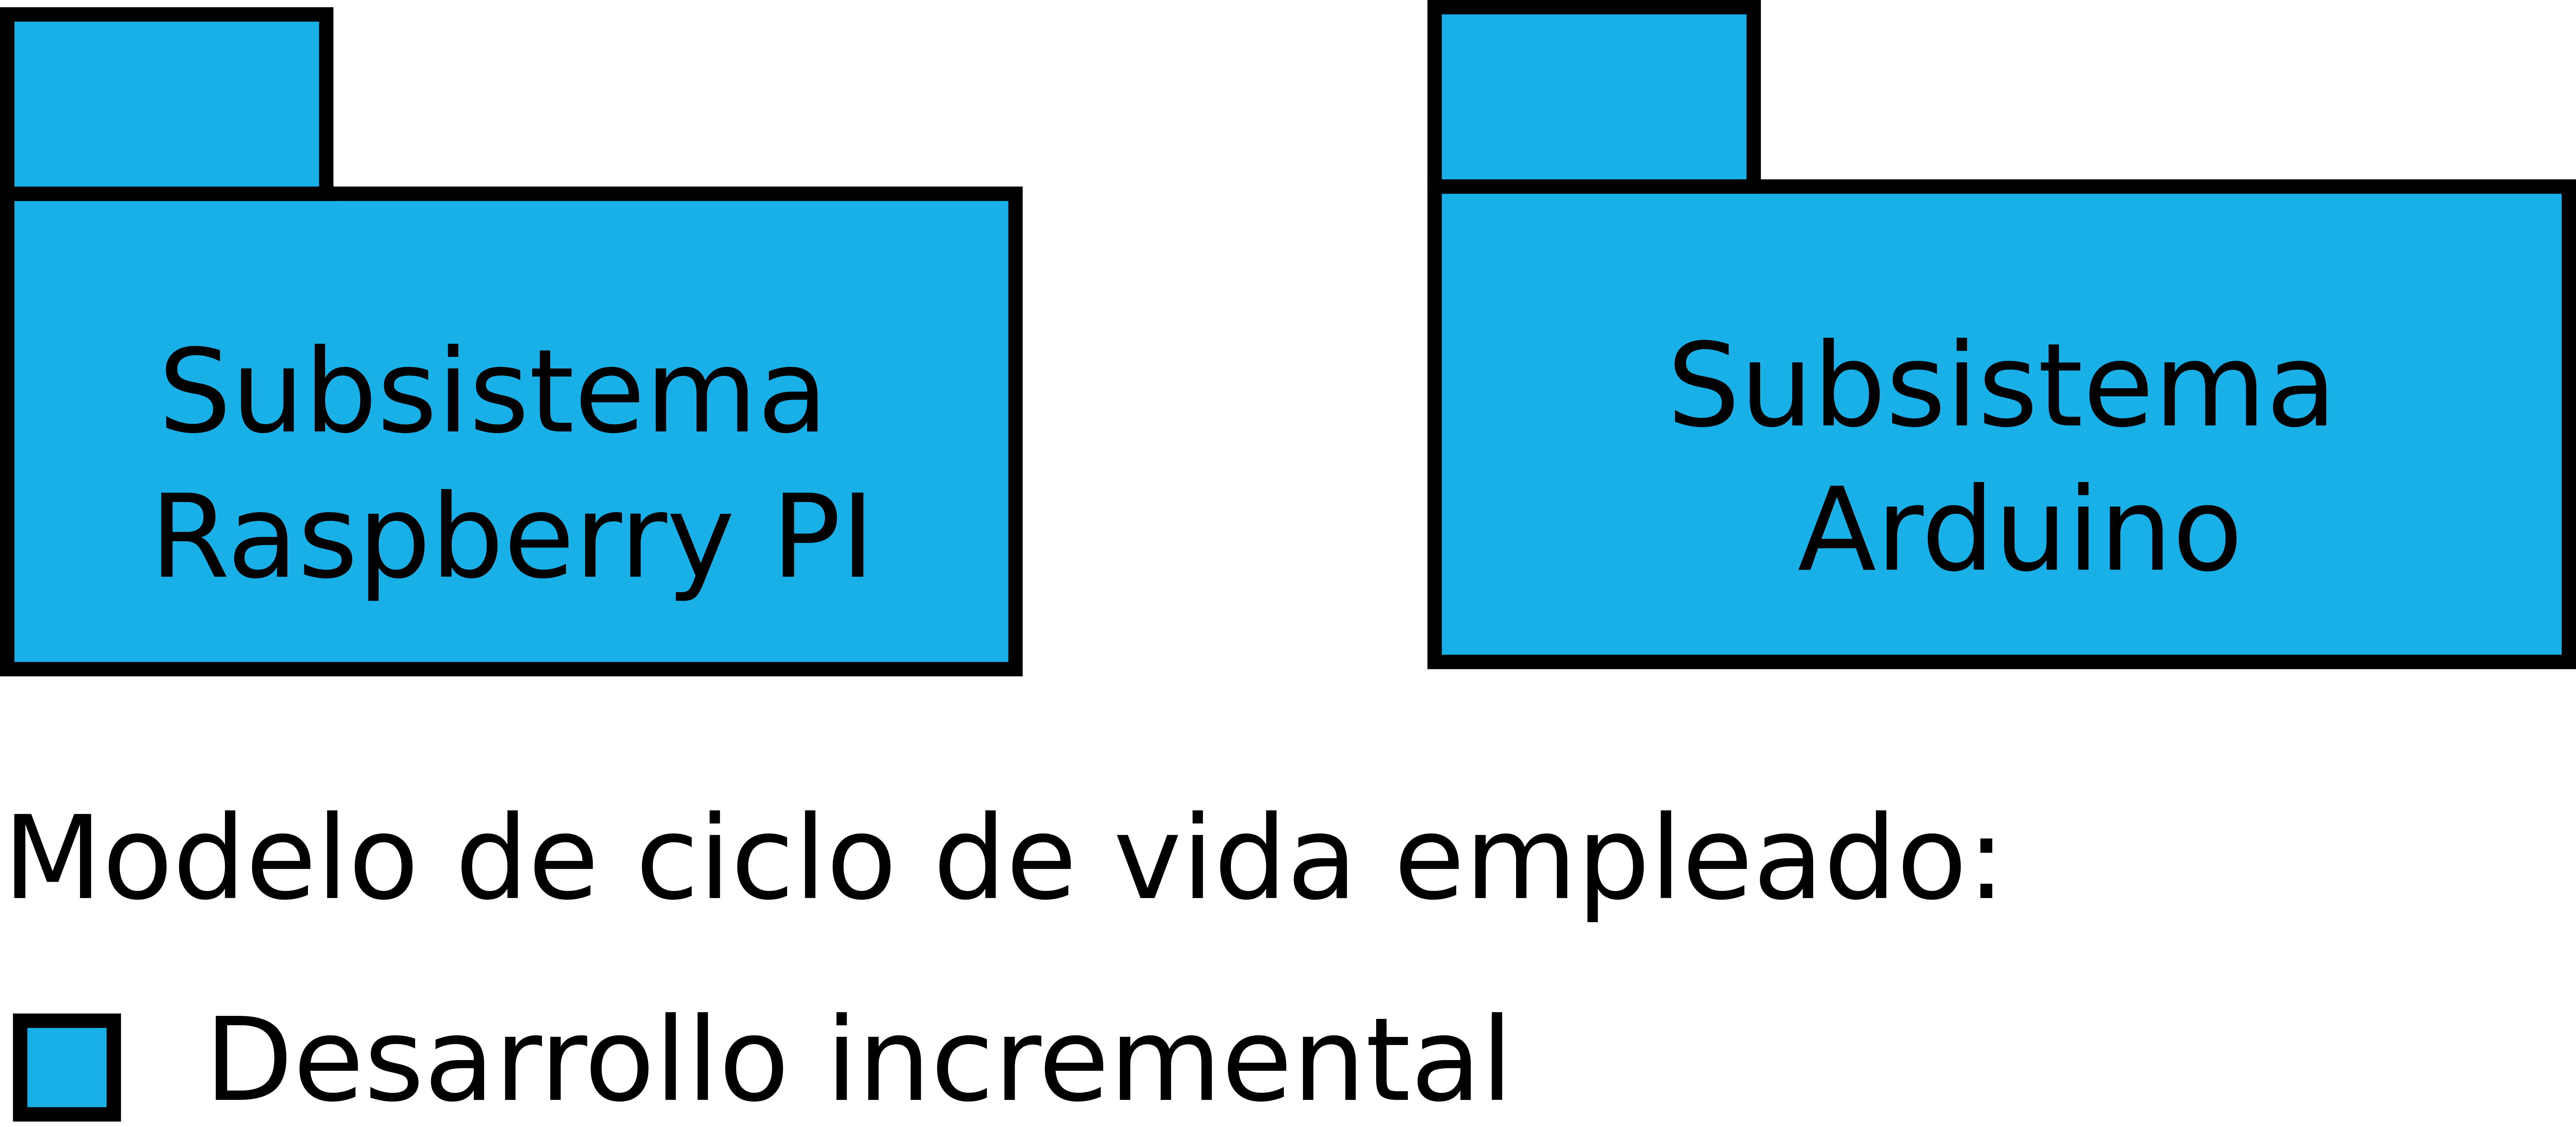
\includegraphics[scale=.6]{diagramas/subsistemas.png}
  \end{center}
  \caption{Subsistemas existentes en el proyecto junto con el modelo de ciclo de vida
utilizado para su desarrollo.}
  \label{website:pagina-principal}
\end{figure}


\section{Recolección de requisitos}

\subsection{Requisitos funcionales}

\subsection{Requisitos no funcionales}



\section {Diagrama de casos de uso}



